\documentclass[ignorenonframetext,]{beamer}
\setbeamertemplate{caption}[numbered]
\setbeamertemplate{caption label separator}{: }
\setbeamercolor{caption name}{fg=normal text.fg}
\beamertemplatenavigationsymbolsempty
\usepackage{lmodern}
\usepackage{amssymb,amsmath}
\usepackage{ifxetex,ifluatex}
\usepackage{fixltx2e} % provides \textsubscript
\ifnum 0\ifxetex 1\fi\ifluatex 1\fi=0 % if pdftex
\usepackage[T1]{fontenc}
\usepackage[utf8]{inputenc}
\else % if luatex or xelatex
\ifxetex
\usepackage{mathspec}
\else
\usepackage{fontspec}
\fi
\defaultfontfeatures{Ligatures=TeX,Scale=MatchLowercase}
\fi
\usetheme{Singapore}
% use upquote if available, for straight quotes in verbatim environments
\IfFileExists{upquote.sty}{\usepackage{upquote}}{}
% use microtype if available
\IfFileExists{microtype.sty}{%
\usepackage{microtype}
\UseMicrotypeSet[protrusion]{basicmath} % disable protrusion for tt fonts
}{}
\newif\ifbibliography
\usepackage{graphicx,grffile}
\makeatletter
\def\maxwidth{\ifdim\Gin@nat@width>\linewidth\linewidth\else\Gin@nat@width\fi}
\def\maxheight{\ifdim\Gin@nat@height>\textheight0.8\textheight\else\Gin@nat@height\fi}
\makeatother
% Scale images if necessary, so that they will not overflow the page
% margins by default, and it is still possible to overwrite the defaults
% using explicit options in \includegraphics[width, height, ...]{}
\setkeys{Gin}{width=\maxwidth,height=\maxheight,keepaspectratio}

% Prevent slide breaks in the middle of a paragraph:
\widowpenalties 1 10000
\raggedbottom

\AtBeginPart{
\let\insertpartnumber\relax
\let\partname\relax
\frame{\partpage}
}
\AtBeginSection{
\ifbibliography
\else
\let\insertsectionnumber\relax
\let\sectionname\relax
\frame{\sectionpage}
\fi
}
\AtBeginSubsection{
\let\insertsubsectionnumber\relax
\let\subsectionname\relax
\frame{\subsectionpage}
}

\setlength{\parindent}{0pt}
\setlength{\parskip}{6pt plus 2pt minus 1pt}
\setlength{\emergencystretch}{3em}  % prevent overfull lines
\providecommand{\tightlist}{%
\setlength{\itemsep}{0pt}\setlength{\parskip}{0pt}}
\setcounter{secnumdepth}{0}
\usepackage{graphicx}
%\usepackage{pgf}
\usepackage{array}
%\usepackage{booktabs}          %% Used in risk tables
%\usepackage{multirow}          %% Used in decision tables
%\usepackage{multicol}          %% Used in the toc
%\usepackage[T1]{fontenc}  %to use < or > in tables
%\usepackage[export]{adjustbox}
\usepackage{tabularx}                                             % table environment providing flexibility
\usepackage{caption}                                              % for creating captions  
\usepackage{longtable}                                            % allows tables to span multiple pages
\usepackage{rotating}                                             % allows for sideways tables
\usepackage{float}                                                % floating environments; may not need in rmarkdown
\usepackage{placeins}                                             % keeps floats from moving
\usepackage{indentfirst}                                          % indents first paragraph of a section
\usepackage{mdwtab}                                               % continued float multi-page figure
\usepackage{enumerate}                                            % create lists
\usepackage{hyperref}                                             % highlight cross references
%\hypersetup{colorlinks=true, urlcolor=blue, linktoc=page, linkcolor=blue, citecolor=blue} %define referencing colors
%\usepackage[usenames,dvipsnames]{xcolor}                          % color name options
%\usepackage[space]{grffile}                                      % spaces in file name path
%\usepackage{soul}                                                 % highlight text
\usepackage{enumitem}                                             % numbered lists
\usepackage{upquote}                                              % produce grave accent in latex
\usepackage{verbatim}                                             % produces verbatim results
\usepackage{fancyvrb}                                             % verbatim in a box
\usepackage{textcomp}                                             % fixes error with packages interfering
\usepackage{lscape}                                               % rotate pages - to allow for landscape longtables
\usepackage{cmap}                                                 % fix mapping characters to unicode

\setbeamersize{text margin left=0.1in}
\setbeamersize{text margin right=0.1in}

\definecolor{pageCol}{rgb}{0.5,0.5,1.0}

\usepackage{tikz}                                                   % used in background


\usebackgroundtemplate{
  \tikz[overlay,remember picture] 
  \node[opacity=0.3, at=(current page.south east),anchor=south east,inner sep=0pt] {
    
\includegraphics[height=0.5in]{noaalogo.jpg}};
}

\setbeamertemplate{footline}
{
  \begin{beamercolorbox}[wd=.05\paperwidth,ht=0ex,dp=0ex,left]{framenumber in head/foot}%
    \insertframenumber/\inserttotalframenumber
    
  \end{beamercolorbox}%
}
\setbeamercolor{footline}{fg=pageCol}

\newcounter{saveenumi}

\title{California Scorpionfish 2017 Assessment}
\subtitle{Biology and Data}
\author{Melissa H Monk\(^1\), \and Xi He\(^1\), \and John Budrick\(^2\)}
\institute{\(^1\)Southwest Fisheries Science Center \and \(^2\)California Department of Fish and Wildlife}
\date{STAR Panel July 24-28, 2017}

\begin{document}
\frame{\titlepage}

\begin{frame}
\tableofcontents[hideallsubsections]
\end{frame}

\begin{frame}

\FloatBarrier

\FloatBarrier

\FloatBarrier
\newpage

\FloatBarrier

\FloatBarrier

\FloatBarrier

\FloatBarrier

\FloatBarrier

\FloatBarrier

\FloatBarrier

\FloatBarrier

\FloatBarrier

\begin{landscape}

\end{landscape}

\FloatBarrier

\newpage

\FloatBarrier

\FloatBarrier

\newpage

\begin{landscape}

\end{landscape}

\newpage

\begin{landscape}

\end{landscape}

\newpage

\begin{landscape}

\end{landscape}

\FloatBarrier

\newpage

\newpage

\FloatBarrier

\end{frame}

\section{Background}\label{background}

\begin{frame}{California scorpionfish \emph{Scorpaena guttata}}

\begin{itemize} 
 \item[\checkmark] Distributed from central California to Punta Eugenia, Baja Mexico  
 \item[\checkmark] Rarely observed north of Pt. Conception  
 \item[\checkmark] Observed from the intertidal to 600 ft,  preferred depth range from 20-450 ft  
 \item[\checkmark] Demersal, found over both hard and soft bottom  
 \item[\checkmark] Exhibit aggregating behavior (spawning and non-spawning)  
\end{itemize}

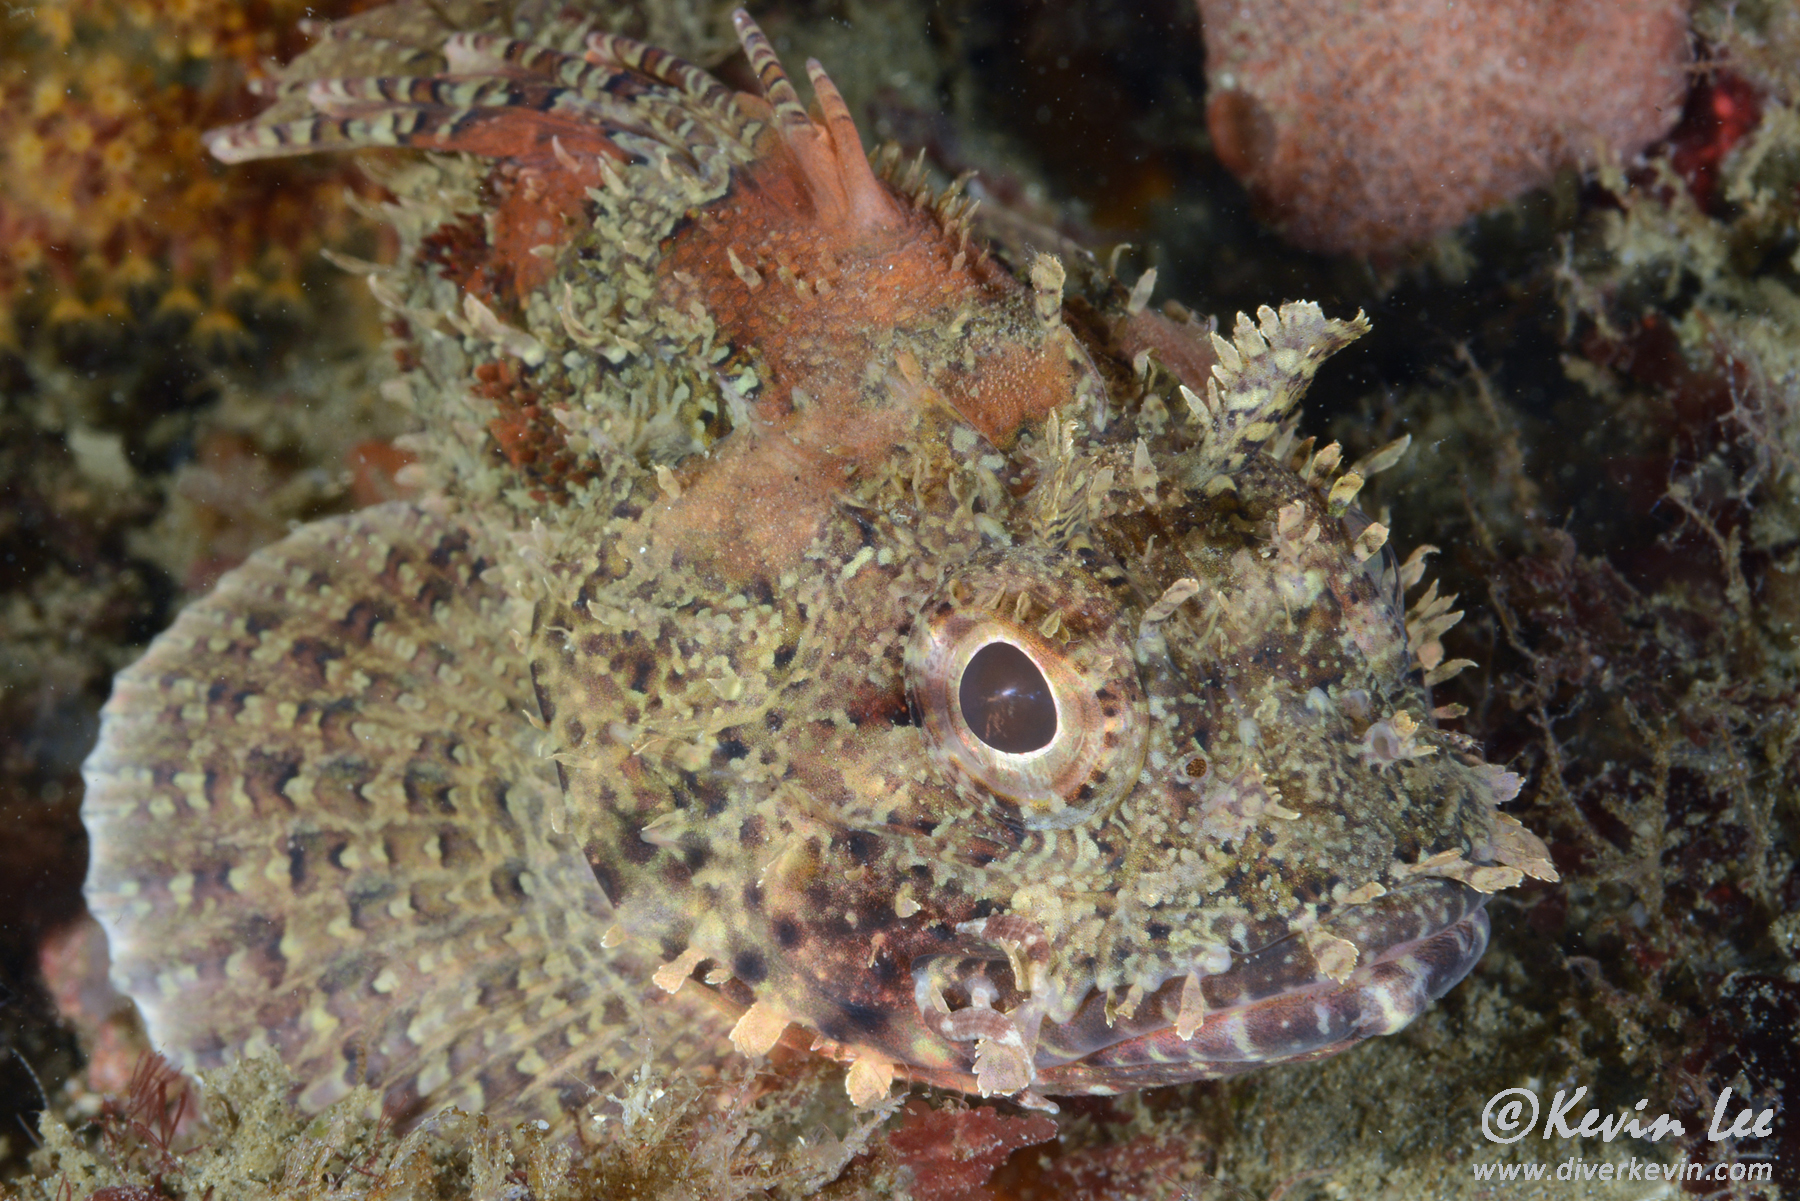
\includegraphics[width=.5\textwidth, inner]{cover_photo}

\end{frame}

\section{Biology}\label{biology}

\begin{frame}{Length-at-age}

\end{frame}

\begin{frame}{Maturity and Fecundity}

\begin{itemize}
\item
  Only information on maturity from Love et al. (1987)
\item
  Found over 50\% of females were mature by 18 cm TL, or two years of
  age.
\item
  All fish were mature by 22 cm TL
\item
  No information available on fecundity of California scorpionfish
\end{itemize}

\end{frame}

\begin{frame}{Weight-at-length}

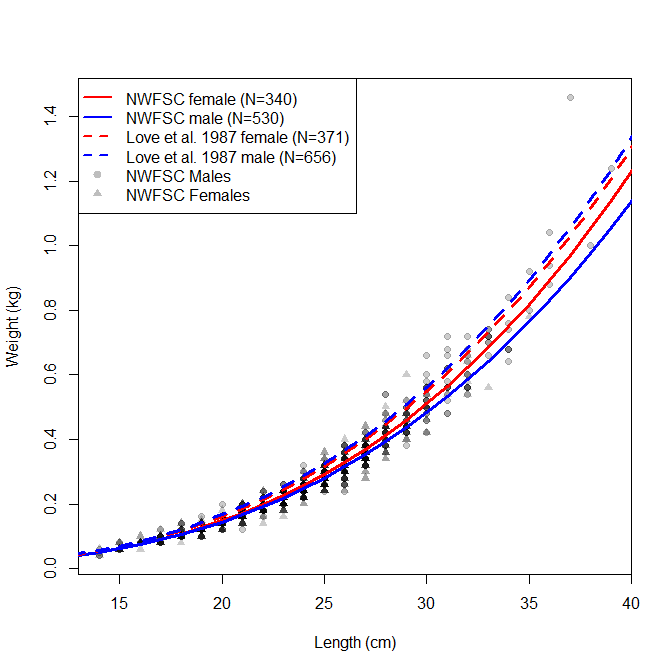
\includegraphics{Figures/Length_weight.png}

\end{frame}

\begin{frame}{Natural mortality}

\end{frame}

\begin{frame}{Steepness}

\end{frame}

\begin{frame}{Summary of Data used in the 2017 Assessment}

\end{frame}

\section{Removals}\label{removals}

\begin{frame}{Total Removals}

\end{frame}

\begin{frame}{Commercial Landings by Fleet}

\end{frame}

\begin{frame}{Recreational Landings by Fleet}

\end{frame}

\section{Index Data}\label{index-data}

\begin{frame}{Summary of Indices}

\begin{itemize}
\tightlist
\item
  All of the methods used to standardize indices have been endorsed by
  the SSC
\end{itemize}

\begin{table}[ht]
\centering
\scalebox{0.7}{
\begin{tabular}{p{2.5in}p{0.8in}p{.4in}p{2in}}
  \hline
Name & Years & Fishery ind. & Method \\ 
  \hline
Recreational PR dockside CPUE & 2004-2016 & No & delta-GLM (bin-lognormal) \\ 
  CPFV logbook CPUE & 1980-2016 & No & negative binomial \\ 
  Onboard observer discard catch CPUE & 2002-2016 & No & delta-GLM (bin-lognormal) \\ 
  Sanitation district CPUE & 1970-2016 & Yes & delta-GLM (bin-lognormal) \\ 
  NWFSC trawl survey CPUE & 2003-2016 & Yes & VAST \\ 
  CSUN/VRG Gillnet survey CPUE & 1995-2008 & Yes & delta-GLM (bin-lognormal) \\ 
  Southern Califrnia Bight trawl survey CPUE & '94, '98, '03, '08, '13 & Yes & delta-GLM (bin-lognormal) \\ 
  Onboard observer retained catch CPUE & 2002-2016 & No & delta-GLM (bin-lognormal) \\ 
   \hline
\end{tabular}
}
\end{table}

\end{frame}

\begin{frame}{Recreational Private Boat Index}

\end{frame}

\begin{frame}{Recreational Party/Charter Boat Index (Logbook)}

\end{frame}

\begin{frame}{Recreational Dead Discard Index}

\end{frame}

\begin{frame}{Recreational Party/Charter Retained Catch Index}

\end{frame}

\begin{frame}{Sanitation Districts Survey Index}

\begin{table}[ht]
\centering
\scalebox{0.9}{
\begin{tabular}{lrrrrr}
  \hline
Program & 0-24 m & 25-49 m & 50-74m & 100+ m & Total \\ 
  \hline
City of Los Angeles & 120 &   0 & 1372 &   0 & 1492 \\ 
  Los Angeles County & 687 &   0 & 5879 & 450 & 7016 \\ 
  Orange County & 161 & 669 & 2157 &  48 & 3035 \\ 
  City of San Diego &   0 & 404 & 333 & 829 & 1566 \\ 
   \hline
\end{tabular}
}
\end{table}

\end{frame}

\begin{frame}{Sanitation Districts Survey Index}

\end{frame}

\begin{frame}{Sanitation Districts Survey Index}

\end{frame}

\begin{frame}{NWFSC Trawl Survey Index}

\end{frame}

\begin{frame}{Gillnet Survey Index}

\end{frame}

\begin{frame}{Southern California Bight Trawl Survey Index}

\end{frame}

\section{Composition Data}\label{composition-data}

\end{document}
